%!TeX encoding = UTF-8 Unicode
%!TeX spellcheck = en-UK
% !TeX root = Perrinet26mnesis.tex
% -*- coding: UTF-8; -*-
%%%-----------------------------------------------------------------
\begin{figure}%[t]
  % \begin{adjustbox}{width=\linewidth}
  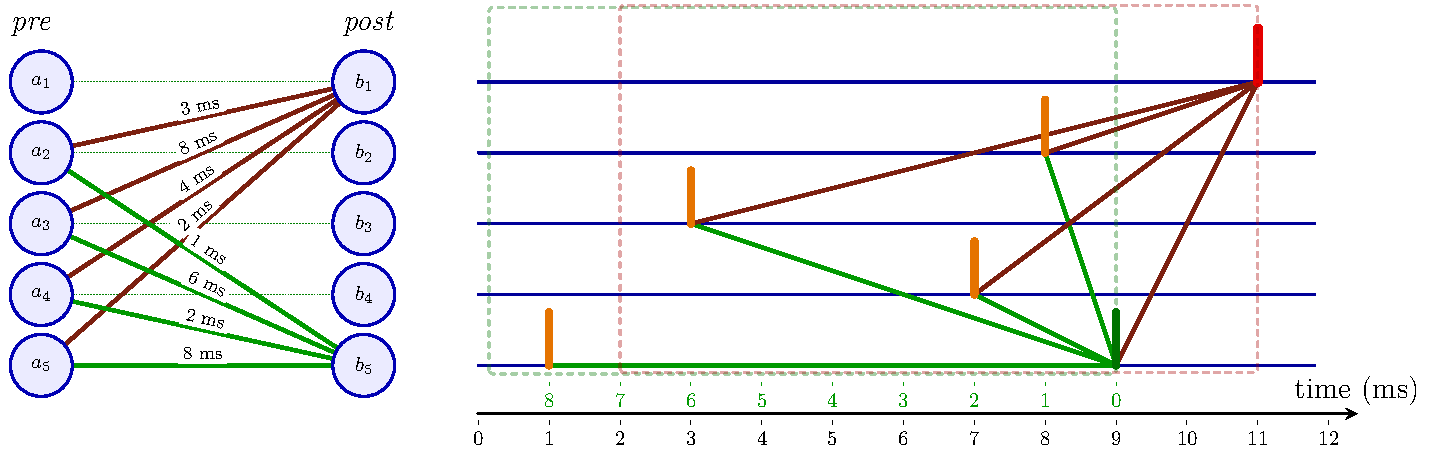
\includegraphics[width=\linewidth]{fig_izhikevich.pdf}%
  % \end{adjustbox}
  \caption{%
    \textbf{Working memory as a chained sequential spike prediction via heterogeneous delays.}
    %
    \emph{Left:} A recurrent HD-SNN of eight neurons numbered $1$--$8$, three of which (faded) take no part in the task, connected by two subsets of recurrent connections that define two Spiking Motifs from the pre-synaptic side (neurons $a$) to the post-synaptic side (neurons $b$): dark-red connections from $a_2$, $a_3$, $a_4$, and $a_5$ target $b_1$ with delays $3$, $8$, $4$, $2$\,ms; green connections from $a_2$, $a_3$, $a_4$, and $a_5$ target $b_5$ with delays $1$, $6$, $2$, $8$\,ms. %
    \emph{Right:} Raster plot of the same two motifs: each trajectory joins an input spike to the spike it contributes to, and faint grey spikes are the spontaneous activity of the inactive neurons.
    %
    \emph{Step~1 --- first prediction (green dashed box):} the orange input spikes emitted at staggered times by $a_2$--$a_5$ within the first context window (dashed green box) constitute a first Spiking Motif. The green delays are tuned so that the four spikes, emitted at $t=8$, $3$, $7$ and $1$\,ms by $a_2$, $a_3$, $a_4$ and $a_5$, converge \emph{synchronously} at $b_5$ at $t=9$\,ms, crossing the firing threshold and producing the green output spike with a precise time. 
    %
    \emph{Step~2 --- second prediction (dark-red dashed box):} the green spike of $b_5$ re-enters the population as a new input of $a_5$. Together with the spikes still visible in the shifted context window (dark-red dashed box), spikes are routed through the dark-red delays in order to converge synchronously on $b_1$ at $t=11$\,ms, generating a new output spike.
    %
    Because output spikes re-enter the same population, detecting one Spiking Motif provides the context for predicting the next spike in the sequence, implementing working memory as a chain of polychronous motifs in which each new temporal prediction is grounded in the preceding context window.
  }
  \label{fig:izhikevich}
\end{figure}
%%%-----------------------------------------------------------------
